%! Author = abenjeddou
%! Date = 30/06/2026

\section{Introduction}
This chapter covers the fifth sprint, focused on packaging the LFU job as a production-ready Docker image, configuring high-availability deployment on Kubernetes, and establishing Flink checkpointing for fault tolerance.

\section{Sprint Goal}

Package the LFU job as a production-ready Docker image, configure high-availability deployment, and establish Flink checkpointing for fault tolerance.

\section{Physical Architecture}

\begin{figure}[!htbp]
    \centering
    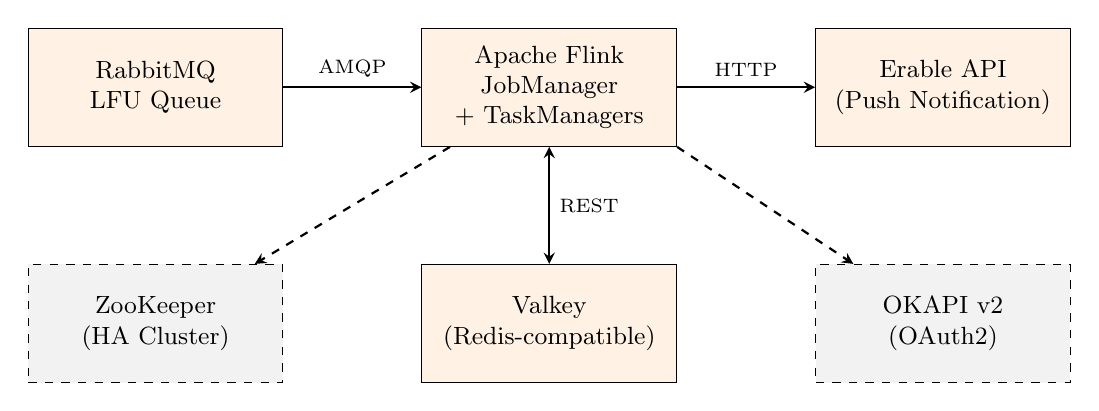
\begin{tikzpicture}[
        node distance=2cm,
        component/.style={rectangle, draw, fill=orange!10, text width=3cm, text centered, minimum height=1.5cm, font=\small},
        infra/.style={rectangle, draw, fill=gray!10, text width=3cm, text centered, minimum height=1.5cm, font=\small, dashed},
        arrow/.style={->, >=stealth, thick}
    ]
% Row 1
        \node[component] (rmq) {RabbitMQ\\LFU Queue};
        \node[component, right of=rmq, xshift=3cm] (flink) {Apache Flink\\JobManager\\+ TaskManagers};
        \node[component, right of=flink, xshift=3cm] (erable) {Erable API\\(Push Notification)};

% Row 2
        \node[infra, below of=rmq, yshift=-1cm] (zk) {ZooKeeper\\(HA Cluster)};
        \node[component, below of=flink, yshift=-1cm] (valkey) {Valkey\\(Redis-compatible)};
        \node[infra, below of=erable, yshift=-1cm] (okapi) {OKAPI v2\\(OAuth2)};

% Arrows
        \draw[arrow] (rmq) -- node[above, font=\scriptsize]{AMQP} (flink);
        \draw[arrow] (flink) -- node[above, font=\scriptsize]{HTTP} (erable);
        \draw[arrow, <->] (flink) -- node[right, font=\scriptsize]{REST} (valkey);
        \draw[arrow, dashed] (flink) -- (zk);
        \draw[arrow, dashed] (flink.south east) -- (okapi);
    \end{tikzpicture}
    \caption{LFU job physical architecture}
    \label{fig:physical-arch}
\end{figure}

\section{Docker Image}

The job is packaged in a Docker~\cite{docker} image based on a customized Flink base image. The \texttt{maven-shade-plugin} produces a fat JAR containing all dependencies (including ONNX Runtime and the embedded AI model).

\begin{lstlisting}[language=bash, caption={Dockerfile (excerpt)}]
FROM pfs-notif-docker.artifactory.../flink_base:1.20.1_scala_2.12_FIX

# Hebex CA certificates for internal APIs (Valkey, Erable, OKAPI)
RUN apt-get install -y hebex-ca-certificates

# Flink dependencies (logback, jackson, slf4j)
COPY flink-dependencies/*logback*.jar $FLINK_HOME/lib/
COPY flink-dependencies/jackson*.jar $FLINK_HOME/lib/
COPY flink-dependencies/slf4j-api-*.jar $FLINK_HOME/lib/

# LFU job fat JAR (including ONNX model in resources)
COPY $job_jar_name $FLINK_HOME/usrlib

# Timezone Europe/Paris for correct log timestamps
RUN ln -snf /usr/share/zoneinfo/Europe/Paris /etc/localtime

# Import Scality S3 certificate into Java keystore
RUN keytool -import -alias ca-s3 \
    -keystore $JAVA_HOME/lib/security/cacerts \
    -file /usr/lib/ssl/certs/root_sha512.pki_orange.pem \
    -storepass changeit -noprompt
\end{lstlisting}

\section{Deployment on Kubernetes}

\subsection{Deployment Environment}
RicKaaStley is a CaaS (Container as a Service) whose purpose is to offer a shared and multi-tenant hosting solution for containerized applications.
It is both a hosting platform and a set of operational services provided on this platform: capabilities to manage metrics, logs, and container orchestration.
The orchestration technology is Kubernetes~\cite{K8S}.

RicKaaStley provides computing resources: CPU, RAM, Network, and Storage, as well as secure, isolated, and sealed environments for each of its clients.
It is a shared and multi-tenant service, meaning that RicKaaStley serves multiple clients isolated from one another: they cannot see each other, do not interact in their consumption of the service, and each is guaranteed the ability to use the resources contracted during subscription.

\subsection{Deployment with Helm}
To deploy our Flink job, we chose to use Helm~\cite{helm} to simplify the lifecycle management of our Flink job.
Helm groups all the YAML files required for deploying our various cluster components into a package called a Chart.

\subsection{Deployed Resources}
Our Helm chart deploys the following Kubernetes resources:

\begin{itemize}
    \item[-] \textbf{A Kubernetes Job object:} manages the JobManager.
    \item[-] \textbf{A Kubernetes Deployment object:} manages the TaskManagers.
    \item[-] \textbf{A Flink-UI service:} exposes the Flink graphical interface to users.
    \item[-] \textbf{A Prometheus service:} exposes metrics so they can be consumed by Prometheus.
    \item[-] \textbf{A ConfigMap:} contains the configuration of our Flink job and will be injected as a YAML file.
\end{itemize}

\section{Flink Cluster Configuration}

The production deployment uses a high-availability architecture:

\begin{itemize}
    \item \textbf{2 JobManagers} in active/passive mode, coordinated via ZooKeeper (3 nodes).
    \item \textbf{3+ TaskManagers} with 2 task slots each (configurable via \texttt{TASK\_MANAGER\_NUMBER\_OF\_TASK\_SLOTS}).
    \item \textbf{Checkpoints} stored on the shared filesystem (\texttt{/opt/flink/checkpoints}).
    \item \textbf{HA metadata} stored in ZooKeeper and the local filesystem (\texttt{/opt/flink/flink-ha}).
\end{itemize}

\section{Checkpointing and Fault Tolerance}

A savepoint is a consistent image of the execution state of a stream processing task, created using Flink's checkpointing mechanism.
We can use savepoints to stop and resume or update our Flink jobs.

\begin{lstlisting}[language=Java, caption={Checkpoint configuration (LFUJob.java)}]
if (CHECKPOINT_ENABLED) {
    env.enableCheckpointing(
        Long.parseLong(CHECKPOINT_INTERVAL_IN_MS), CHECKPOINTING_MODE);
    env.getCheckpointConfig()
       .setMinPauseBetweenCheckpoints(MIN_PAUSE_BETWEEN_CHECKPOINTS);
    env.getCheckpointConfig()
       .setCheckpointTimeout(CHECKPOINT_TIMEOUT_IN_MS);
    env.getCheckpointConfig()
       .setMaxConcurrentCheckpoints(MAX_CONCURRENT_CHECKPOINTS);
    env.getCheckpointConfig()
       .setExternalizedCheckpointCleanup(EXTERNALIZED_CHECKPOINT_CLEANUP);
}
\end{lstlisting}

\begin{itemize}
    \item \textbf{Mode}: \texttt{EXACTLY\_ONCE} (default) or \texttt{AT\_LEAST\_ONCE} (required for correlation ID).
    \item \textbf{Interval}: Configurable (default 1000~ms in dev, 10000~ms in integration).
    \item \textbf{Externalized checkpoints}: Retained after job cancellation to allow restart from the last consistent state.
    \item \textbf{Compression}: Optional snapshot compression to reduce storage overhead.
\end{itemize}

\section{Rebalance Strategy}

Each operator is followed by a \texttt{.rebalance()}, ensuring round-robin distribution of the stream across parallel instances. This avoids \textit{hot spots} when certain MSISDNs generate disproportionately more events than others.

\section{Continuous Integration Pipeline}

The CI/CD pipeline triggers each time a commit is made to the main branch. It is divided into three stages:

\begin{enumerate}
    \item \textbf{Build:} Compiles the Java source code and produces a JAR stored in the job's artifacts. During this stage, unit and integration tests are executed to ensure that no regression has been introduced.

    \item \textbf{Analysis:} This stage contains two jobs:
    \begin{itemize}
        \item[-] \textbf{Fortify:} is a security-oriented static analysis tool that identifies potential security vulnerabilities in the source code.
        \item[-] \textbf{Sonar:} is a tool dedicated to continuous inspection of source code quality. It offers advanced static code analysis features to identify bugs, vulnerability risks, poor coding practices, and to evaluate test coverage.
    \end{itemize}

    \item \textbf{DockerBuild:} Responsible for building the Docker image. It depends on the build job, which prepares the JAR so it can be integrated into the Docker image, then pushed to the Artifactory. This subsequently allows retrieving the image for deployment.
\end{enumerate}

\section{Environment Variables}

\begin{table}[!htbp]
    \centering
    \caption{Main environment variables}
    \label{tab:env-vars}
    \begin{tabularx}{\textwidth}{l c X}
\toprule
\textbf{Variable} & \textbf{Default} & \textbf{Description} \\
\midrule
\multicolumn{3}{l}{\textit{RabbitMQ Source}} \\
\texttt{RMQ\_LFU\_QUEUE} & --- & RabbitMQ queue name \\
\texttt{RMQ\_HOST} & --- & RabbitMQ broker host \\
\texttt{USE\_CORRELATION\_ID} & false & Enable correlation ID tracking \\
\midrule
\multicolumn{3}{l}{\textit{Flink}} \\
\texttt{GLOBAL\_PARALLELISM} & 1 & Global job parallelism \\
\texttt{CHECKPOINT\_ENABLED} & false & Enable checkpointing \\
\texttt{CHECKPOINT\_INTERVAL\_IN\_MS} & 1000 & Interval between checkpoints (ms) \\
\texttt{CHECKPOINT\_MODE} & EXACTLY\_ONCE & Checkpointing mode \\
\texttt{USE\_SNAPSHOT\_COMPRESSION} & false & Snapshot compression \\
\texttt{LATENCY\_INTERVAL} & --- & Latency tracking interval \\
\midrule
\multicolumn{3}{l}{\textit{Valkey}} \\
\texttt{VALKEY\_HOST\_HTTP} & --- & Valkey API URL \\
\texttt{VALKEY\_BASE\_PATH} & /pns/v3/users & API base path \\
\midrule
\multicolumn{3}{l}{\textit{Erable}} \\
\texttt{ERABLE\_HOST} & --- & Erable service URL \\
\texttt{ERABLE\_STUBBED} & false & Stub mode (testing) \\
\midrule
\multicolumn{3}{l}{\textit{Artificial Intelligence}} \\
\texttt{AI\_ANOMALY\_THRESHOLD} & 0.85 & Anomaly detection threshold \\
\texttt{AI\_MODEL\_PATH} & /models/fairuse\_prediction.onnx & ONNX model path \\
\bottomrule
    \end{tabularx}
\end{table}

\section*{Conclusion}

At the end of Sprint~5, the LFU job was deployable as a Docker container on Kubernetes with full high-availability support. The CI/CD pipeline produced the fat JAR, built the Docker image, and pushed it to the Artifactory registry. Checkpoint recovery was validated by simulating TaskManager failures.

